% !TEX encoding = UTF-8
% !TEX TS-program = pdflatex
% !TEX root = ../Tesi.tex
% !TEX spellcheck = it-IT

%************************************************
\chapter{Ethereum}
\label{ethereum-chapter}
%************************************************
In questo capitolo andremo ad approfondire Ethereum, una delle alt-chain in circolazione dopo la comparsa di bitcoin. Ethereum è una piattaforma che processa ed esegue smart contract Turing-completi basandosi su di un libro mastro blockchain. Non è un clone di Bitcoin ma bensì una nuova implementazione dal design completamente indipendente. Anche se, come alt-chain, non è tenuto ad esserne provvisto, Ethereum ha una propria moneta integrata, chiamata \textit{ether}, richiesta per pagare l'esecuzione di un contratto. La blockchain Ethereum registra i vari contratti che sono espressi in un linguaggio Turing-completo di basso livello. Uno smart contract è sostanzialmente un programma che gira su ogni nodo del sistema Ethereum. Tali contratti possono memorizzare dati, inviare / ricevere pagamenti in ether, memorizzare ether, ed eseguire una gamma infinita di azioni calcolabili, agendo come agenti decentralizzati di software autonomo.

\section{Introduzione}
Ethereum è spesso descritto come "the world computer". Dal punto di vista informatico Ethereum è una macchina a stati deterministica ma praticamente illimitata, costituita da uno stato sigleton accessibile a livello mondiale ed una propria macchina virtuale \textit{EVM} che applica le modifiche a tale stato. E' un'infrastruttura open source, globalmente decentralizzata sviluppata per eseguire programmi denominati \textit{smart contract}. Utilizza la blockchain per sincronizzare e memorizzare le modifiche di stato del sistema, assieme ad una criptovaluta chiamata \textit{ether} utilizzata per limitare le risorse per l'esecuzione dei contratti. 
Diversamente da Bitcoin, che ha un linguaggio di scriptiong molto limitato, Ethereum è stato concepito per essere una blockchain programmabile per l'uso generico che esegue una macchina virtuale in grado di eseguire codice di complessità arbitraria ed illimitata. Il linguaggio script di Bitcoin è stato intenzionalmente vincolato a delle semplici valutazioni true / false delle condizioni di spesa, il linguaggio di Ethereum invece risulta Turing-completo, può infatti funzionare come un general-purpose computer.

\subsection*{La nascita di Ethereum}
Ethereum è stato concepito in un momento in cui le persone hanno riconosciuto la potenza di un modello quale Bitcoin e stavano cercando di andare oltre alle applicazioni di criptovaluta. L'enigma principale era: costruire su Bitcoin o avveriare una nuova blockchin? Costruire al di sopra di Bitcoin significava vivere entro gli intenzionali limiti imposti da tale rete cercando soluzioni alternative. L'insieme limitato di tipologia di dati e dimensione della memorizzazione di questi sembrava limitare il numero di applicazioni che potevano essere eseguite su bitcoin, qualsiasi ulteriore aggiunta avrebbe implicato la nacessità di implementare ulteriori strati fuori catena, anullando così molti dei vantaggi nell'uso di una blockchain pubblica. Per tale progetto si necessitava di maggiore libertà e fluidità rimanendo on-chain, l'unica opzione era una nuova blockchain.
Verso la fine del 2013, Vitalik Buterin, un giovane programmatore apassionato di Bitcoin, pensò di estendere le capacità di Bitcoin e Mastercoin. Nell'ottobre di quell'anno, propose un approccio più generalizzato al team di Mastercoin, che consentiva contratti flessibili e programmabili, anche se non Turing-completi, in sostituzione dell'allora attuale linguaggio contrattuale di Mastercoin, ma questa proposta risultava una modifica troppo radicale er adattarsi alla loro roadmap di sviluppo. 
Nel dicembre 2013, Vitalik condivise un white paper che delineava l'idea di Ethereum: una blockchain Turing-completa per tutti gli usi. Si aggiunse al team  il Dr. Gavin Wood, attuale CTO, che lo aiutò nel perfezionale il protocollo che attualmente porta il nome di Ethereum. 
Lo sviluppo di Ethereum è stato pianificato in quattro fasi distinte, con importanti cambiamenti in ciascuna fase. Ogni fase può includere delle subreleases, note come "hard fork", che apportando funzionalità non retro compatibili. Le quattro fasi di sviluppo portano il nome di \textit{Frontier, Homestead, Metropolis, Serenity}. I fork intermedi programmati sono \textit{Ice Age, DAO, Tangerine Whistle, Spurious Dragon, Byzantinum e Costantinople}. L'elenco completo lo possiamo notare in Tabella~\ref{tab:fork-intermedi}.
%
\begin{table}[]
	\centering
	\begin{tabular}{|c|p{10cm}|}
		\hline
		\textbf{Numero blocco} & \textbf{Descrizione} \\ \hline
		\lstinline|Blocco #0| & Frontier - Fase iniziale di Ethereum, 30 luglio 2015 - marzo 2016.\\ \hline
		\lstinline|Blocco #200000| & Ice Age - Hard fork per introdurre un aumento di difficoltà esponenziale, per motivare la futura transazione verso PoS.\\ \hline
		\lstinline|Blocco #1150000| & Homestead - Seconda fase di Ethereum lanciata a marzo 2016.\\ \hline
		\lstinline|Blocco #1192000| & DAO - Hard fork che ha rimborsato le vittime del contratto DAO hacked causando la separazione di Ethereum ed Ethereum Classic.\\ \hline
		\lstinline|Blocco #2463000| & Tangerine Whistle - Hard fork per modificare il calcolo del gas per certa operazioni di I/O.\\ \hline
		\lstinline|Blocco #2675000| & Spurious Dragon - Hard fork per sventare vettori d'attacco DoS e meccanismi di protezione ai replay attack.\\ \hline
		\lstinline|Blocco #4370000| & Metropolis Byzantium - Terza tappa di Ethereum lanciata nell'ottobre 2017.\\ \hline
	\end{tabular}
	\caption{Fork intermedi della blockchain Ethereum}
	\label{tab:fork-intermedi}
\end{table}
Dopo Byzantium, rimangono altri due hard fork Metropolis Costantinople ed a seguire la fase finale Serenity.

\subsection{Turing-completezza di Ethereum}
La capacità di Ethereum di eseguire un programma memorizzato, in un macchina a stati chiamata Ethereum Virtual Machine, mentre legge e scrive dati in memoria lo rende un sistema Turing Completo. Ethereum può infatti calcolare qualsiasi algoritmo che possa essere calcolato da qualunque macchina di Turing.
L'innovativa invenzione di Ethereum consiste nel combinare l'architettura di calcolo generica di un computer con l'affiancamento di una blockchai decentralizzata che memorizza il programma da eseguire. In questo modo si crea un computer mondiale distribuito (singleton). I programmi Ethereum funzionano ovunque producendo uno stato comune che viene garantito dalle regole di consenso. 
Il fatto che Ethereum si turing completo porta con se una conseguente problematica, il fatto che possa eseguire qualsiasi programma, di qualsiasi complessità. Questa flessibilità porta alcuni problemi dal punto di vista della sicurezza e di gestione delle risorse disponibili. 
Turing ha dimostrato che non è possibile prevedere se un programma terminerà o meno senza eseguirlo. Ciò pone una sfida: ogni nodo partecipante (client) dovrà convalidare ogni singola transazione, convalidando qualsiasi smart contract che chiama, ma come dimostrato da Turing, Ethereum non potrà sapere a priori se uno smart contract terminerà, o per quanto tempo verrà eseguito, senza effettivamente eseguirlo. Se per caso o di proposito fosse possibile creare un contratto facendo in modo che funzioni per sempre quando un nodo tenterà di convalidarlo si verificherebbe un attacco di tipo DoS. Per evitare che questo accada Ethereum introduce un meccanismo di misurazione delle risorse chiamato \textit{gas}. Quando l'EVM esegue uno smart contract tiene accuratamente conto di ogni istruzione (calcolo, accesso ai dati, ecc \dots). Ogni istruzione ha un proprio costo predeterminato in \textit{gas}. Quando una transazione attiva l'esecuzione di un contratto, deve includere una quantità di \textit{gas} che imposta come limite superiore di ciò che può essere consumato eseguendo tale smart contract. Le unità di gas devono essere incluse quindi acquistate con l'ether, durante il calcolo della transazione.

\subsection{Dalla Blockchain generica alle \DH Apps}
Ethereum è nato con l'intenzione di creare una blockchain general-purpose che potesse essere programmata per svariati usi. Molto rapidamente la visione di Ethereum si è espansa fino a diventare una piattaforma per programmare DApps. Queste DApps presentano una prospettiva più ampia rispetto agli smart contract. Una DApp è come minimo un contratto munito però di un'interfaccia web utente. Più in generale, una DApp è un'applicazione Web costruita su servizi di un'infrastruttura aperta, decentralizzata e peer-to-peer. Lo si può anche trovare scritto in questo modo \DH App. Il carattere \DH rappresenta il carattere latino \textit{ETH} che appunto allude a Ethereum.

\subsection{Le unità monetarie di Ethereum}
L'unità monetaria di Ethereum si chiama \textit{ether} ed è identificata con il nome di \textit{ETH}. Un ether è suddiviso in unità più piccole, fino all'unità più piccola chiamata \textit{wei}. All'interno di Ethereum il valore di \textit{ether} viene sempre rappresentato in \textit{wei}. Le denominazioni delle varie frazioni di ether hanno sia un nome scientifico che utilizza il sistema internazionale di unità, SI, sia un nome colloquiale che rende omaggio a molte delle più grandi menti della matematica e della crittografia, tutte le denominazioni sono riportate in Tabella \ref{tab:frazioni-di-ether}.
\begin{table}[]
	\centering
	\begin{tabular}{|l|c|c|c|}
		\hline
		\textbf{Valore (in wei)}			& \textbf{Esp.}	& \textbf{Nome} & \textbf{Nome \textit{SI}}\\ \hline
		1 									&	$1$			&	wei			&	Wei\\ \hline
		1.000 								&	$10^{3}$	&	Babbage		&	Kilowei o femtoether\\ \hline
		1.000.000 							&	$10^{6}$	&	Lovelace	&	Megawei o picoether\\ \hline
		1,000,000,000						&	$10^{9}$	&	Shannon		&	Gigawei o nanoether\\ \hline
		1.000.000.000.000					&	$10^{12}$	&	Szabo		&	Microetere o micro\\ \hline
		1.000.000.000.000.000				&	$10^{15}$	&	Finney		&	Milliether o milli\\ \hline
		1.000.000.000.000.000.000			&	$10^{18}$	&	Ether		&	Ether\\ \hline
		1.000.000.000.000.000.000.000		&	$10^{21}$	&	Grand		&	Kiloether \\ \hline
		1.000.000.000.000.000.000.000.000	&	$10^{24}$	&				&	Megaether \\ \hline
	\end{tabular}
	\caption{Denominazioni delle frazioni di ether.}
	\label{tab:frazioni-di-ether}
\end{table}

\subsection*{Wallet}
Il termine wallet rappresenta tutti quei software che aiutano l'utente nella gestione del proprio account Ethereum, memorizza infatti le chiavi d'accesso ai fondi, crea e trasmette transazioni. Esistono varie tipologie di wallet, che richiedono più o meno attenzione per la gestione delle chiavi, più controllo e indipendenza si vuole avere, più aumentano le responsabilità. Un buon wallet è per esempio MetaMask, portafoglio web-based che si presenta come un'estensione per i browser più comuni come Chrome, Firefox e Opera. Risulta facile da usare e conveniente per eseguire test, poichè risulta in grado di connettersi ad una vasta gamma di nodi Ethereum per testare la blockchain. L'installazione di MetaMask risulta veramente semplice, infatti basterà aprire il gestore estensioni del proprio browser e cercare tale estensione e una volta individuata procedere con l'istallazione. Al termine della procedura si aprirà automaticamente la schermata principale di MetaMask dove ci viene richiesto di inserire una password. Tale password servirà per impedire a chiunque utilizzi il computer in questione e quindi ha accesso al browser su cui è installato MetaMask, di accedere a tale wallet e quindi aver accesso ai fondi. A questo punto viene generato un backup mnemonico formato da 12 parole inglesi. Queste parole potranno essere utilizzate in qualsiasi wallet compatibile per recuperare l'accesso al proprio conto in caso di guasti di qualsiasi tipo. Si consiglia di conservare un backup cartaceo delle credenziali d'accesso e del backup mnemonico riponendolo in un luogo fisicamente sicuro. Si sconsiglia infatti di salvare digitalmente tali informazioni.
A questo punto ci troveremo davanti ad una schermata dove ci viene mostrato il nostro conto. Troviamo varie informazioni tipo il nostro indirizzo casualmente generato, il saldo del conto, lo storico delle transazioni passate e in corso. In questa schermata sarà anche possibile selezionare la rete sulla quale inviare le nostre transazioni. Le varie reti disponibili sono:
\begin{itemize}
	\item \textbf{Rete principale di Ethereum:} principale blockchain pubblica di Ethereum, in questa rete il valore in ether è reale e ogni azione avrà conseguenze reali.
	\item \textbf{Rete di test Ropsten:} rete con blockchain pubblica in cui ether non ha valore.
	\item \textbf{Rete di test Kovan:} rete con blockchain pubblica in cui ether non ha valore. Utilizza il protocollo di consenso Aura. Questa rete è supportata solo da Parity, gli altri client il protocollo di consenso Clique, proposto in seguito. 
	\item \textbf{Rete di test Rinkeby:} rete con blockchain pubblica, utilizza il protocollo di consenso Clique. Anche in questa rete Ether non ha valore.
	\item \textbf{Localhost 8545:} Si connette ad un nodo in esecuzione sullo stesso computer del browser. Tale noto può far parte di una blockchain pubblica o di una rete di test privata.
	\item \textbf{RPC personalizzata:} consente di collegare MetaMask a qualsiasi nodo con un'interfaccia \textit{RPC} (Remote Procedure Call) compatibile con Geth. Tale nodo può essere parte di una blockchain pubblica o privata. 	
\end{itemize}
Prenderemo come esempio la \textit{rete di test Ropsten}.

Per muovere i primi passi su Ethereum, o qualsiasi altra blockchain, abbiamo bisogno di fondi. Per eseguire dei test possiamo richiedere dei fondi gratuitamente sulle reti di test, per esempio Ropsten. Quindi da MetaMask selezioniamo la sopracitata rete di test selezioniamo \textit{Deposita > Ottieni Ether}, a questo punto si aprirà un'altra scheda dove poter richiedere \textit{1 ether from faucet}. Una volta eseguita la richiesta, in basso, nella sezione \textit{transactions} comparirà l'ID della transazione appena eseguita per trasferire 1 ether sul nostro conto. Attendendo qualche secondo la somma richiesta vi verrà accredita e possiamo effettuare dei pagamenti. Per fare ciò dobbiamo tenere conto del \textit{gas}, commissione raccolta dai minatori per convalidare la transazione. Il costo massimo corrisponde a :
\[ 3*21000 \text{ gwei} \quad = \quad 63000 \text{ gwei} \quad = \quad 0.000063 \text{ ETH}\]
Questo sta a significare che una transazione di $ 1 \text{ ETH} $ costerà $ 1.000063 \text{ ETH} $, nonostante MetaMask visualizzi cifre approssimate, omettendo di visualizzare le cifre meno significative, sia nel saldo del conto che nel totale delle singole transazioni.

Durante la presentazione di Ethereum abbiamo anticipato che una delle particolarità di questa nuova blockchain sta proprio nella possibilità implementazione di smart contract da sottomettere al computer mondiale Ethereum. Vediamo ora come creare il primo contratto che ci darà la possibilità di depositare ether sul conto del contratto creato e successivamente procedere con il prelievo di massimo 0.1 ether. Il contratto che andremo a creare si chiama \textit{faucet} e verrà scritto in Solidity tramite Remix\footnote{Remix è un IDE per la scrittura di Smart Contract in linguaggio Solidity, tramite browser. http://remix.ethereum.org}. Il funzionamento di questo contratto è semplice: distribuisce ether a qualsiasi indirizzo che ne richiede e il conto di tale contratto può essere caricato periodicamente. Per procedere quindi dobbiamo copiare il codice qui riportato all'interno di un nuovo file \textit{faucet.sol} all'interno di Remix. A questo punto l'IDE compilerà in automatico mostrando un riquadro verde riportante il nome del contratto. Ora siamo pronti per inviare questo smart contract sulla blockchain pubblica e successivamente testarlo.
\begin{lstlisting}
// Our first contract is a faucet!
pragma solidity ^0.4.19;

contract Faucet {
   // Give out ether to anyone who asks
   function withdraw(uint withdraw_amount) public {
      // Limit withdrawal amount
      require(withdraw_amount <= 100000000000000000);	■\label{line:max_amount}■
      // Send the amount to the address that requested it
      msg.sender.transfer(withdraw_amount);
   }
   // Accept any incoming amount
   function () public payable {}
}
\end{lstlisting}
La registrazione di un contratto sulla blockchain comporta la creazione di una transazione speciale la cui destinazione è l'indirizzo $0\text{x}000 \dots 000$ noto come indirizzo zero, facendo capire alla blockchain Ethereum che siamo intenzionati a registrare un nuovo smart contract. Fortunatamente Remix riesce ad interagire con MetaMask, semplicemente impostando la voce in \textit{Run > Environment} sul valore \textit{Injected Web3 - Ropsten}. Subito al di sotto di questa voce troviamo la voce \textit{Deploy} che procederà con la creazione di una nuova transazione che portando alla registrazione del contratto. Una volta confermata tale transazione possiamo richiamare la funzione \textit{withdraw(uint withdraw\_amount)} inserendo massimo 0.1 ETH, limite impostato alla riga \ref{line:max_amount}, nell'apposito campo della scheda Run, vista in precedenza e procedere premendo il pulsante \textit{transact}. A questo punto verrà creata una nuova transazione verso l'indirizzo del contratto richiedendo tale somma di ether. Se tutto andrà a buon fine, il contratto esaminerà tale richiesta e produrrà un'ulteriore transazione trasferendo la cifra indicata verso il nostro conto. Si consiglia di utilizzare https://ropsten.etherscan.io per visualizzare tutti i dettagli delle varie transazioni, una cosa importante da notare è il fatto che le transazioni di risposta di contratti non vengono riportate nel tab \textit{Transaction}, ma compariranno nel tab \textit{Internal Txns}.

\section{Le transazioni}
Le transazioni sono messaggi firmati originati da un account di proprietà che vengono trasmessi della rete Ethereum e registrati sulla blockchain. La struttura di base di una transazione è quella che vediano in tabella \ref{tab:struttura_base_transazioni}.
%
\begin{table}[]
	\centering
	\begin{tabular}{|c|p{11cm}|}
		\hline
		\textbf{Campo} & \textbf{Descrizione} \\ \hline
		nonce & Numero di sequenza emesso dall'EOA di origine, utilizzato per impedire il replay attack.\\ \hline
		gas price & Prezzo del gas in wei che il mittente è disposto a pagare.\\ \hline
		gas limit & Quantità massima di gas che l'EOA di origine è disposto ad acquistare per la transazione corrente.\\ \hline
		recipient & Indirizzo Ethereum a cui è destinata la transazione. \\ \hline
		value & Quantità di ether da inviare a destinazione.\\ \hline
		data & Lunghezza variabile del payload.\\ \hline
		v, r, s & Tre componenti della firma digitale ECDSA dell'EOA di origine.\\ \hline
	\end{tabular}
	\caption{Struttura base di una transazione Ethereum.}
	\label{tab:struttura_base_transazioni}
\end{table}
%
La struttura del messaggio transazione viene serializzata utilizzando lo schema di codifica RLP (Recursive Length Prefix), creato appositamente per semplificare la serializzazione dei dati in Ethereum. Tutti i numeri vengono codificati come interi big-endian, di lunghezze che sono multipli di 8 bit. Le etichette di campo non fanno parte dei dati serializzati della transazione, che contiene valori di campo codificati in RLP. In generale RLP non contiene alcun delimitatore o etichetta di campo e la lunghezza di ciascun campo viene identificata tramite un prefisso. Molte informazioni visualizzate da wallet e altri strumenti sono derivate da altre più primitive. Per esempio la chiave pubblica dell'EOA può essere ricavata dalle componenti \textit{v, r, s} della firma ECDSA.

\subsection*{Nonce}
Il nonce è uno dei componenti più importanti ma meno comprese in Ethereum. La definizione che troviamo nel White Paper si legge: \textit{"nonce: numero scalare uguale al numero di transazioni inviate da questo indirizzo, o nel caso di account con codice associato, il numero di creazioni di contratto effettuate da questo account"}. Esistono due scenari in cui l'esistenza di un nonce risulta importane.
\begin{enumerate}
	\item Supponiamo di aver due transazioni da effettuare, una puù importante dell'altra ma non disponiamo di un saldo sufficiente per pagare entrambe le transazioni. Se inviassimo, in un sistema decentralizzato come Ethereum, prima la transazione più importente e poi la seconda, non disponendo del campo nonce, non abbiamo la certezza che la prima transazione venga sicuramente eseguita prima dell'altra, dato che i nodi possono ricevere le transazioni in entrambi gli ordini.
	\item Immaginiamo ora di possedere un portafoglio Ethereum con parecchi fondi, e di fare un trasferimento di pochi ether ad un altro indirizzo. Senza il campo nonce un qualsiasi altro untente che vede tale transazione la potrà replicare fintanto chè sul nostro conto abbiamo fondi a sufficienza da coprire la cifra versata.
\end{enumerate}
Il campo nonce ha un duplice scopo, dare un ordine di esecuzione alle transazioni, sostanzialmente l'ordine di creazione, ed essendo unico, serve a sventare i replay attack.

\subsection{Gas di transazione}
Come abbiamo già detto precedentemente, il gas è il carburante di Ethereum, una valuta virtuale separata da l'ether con il proprio tasso di cambio. Ethereum utilizza il gas per controllare la quantità di risorse che una transazione può utilizzare dal momento che il modello di calcolo a terminazione aperta (Turing completo) richiede una qualche forma di misurazione al fine di evitare attacchi di denial-of-service. Il gas è separato dall'ether per proteggere il sistema dalla volatilità che potrebbe insorgere assieme ai rapidi cambiamenti nel valore dell'ether. Il cambio gas / ether può quindi variare al valiare del valore della valuta ether. 

Il campo getPrice in una transazione consente all'ordinante di impostare il prezzo che è disposto a pagare in cambio del gas. Il prezzo è misurato in wei per unità di gas. I wallet possono regolare il prezzo del gas nelle transazioni per ottenere una conferma più rapida, maggiore sarà il prezzo del gas, più rapida sarà la conferma della transazione. Il valore minimo a cui getPrice può essere impostato è zero. Queste transazioni risulteranno quindi completamente gratuite ma rischiano di non essere mai confermate. 

Se l'indirizzo di destinazione è uno smart contract, la quantità di gas può essere stimata ma non può essere determinata con precisione. Questo perchè un contratto può valutare diverse condizioni che portano a diversi percorsi di esecuzione, con conseguenti costi totali di gas diversi. 

\subsection*{Destinatario della transazione}
Il destinatario della transazione viene specificato nel campo \textit{to}. Questo contiene un indirizzo Ethereum di 20 byte che può essere un EOA o un indirizzo di un qualche contratto. Ethereum con convalida ulteriormente questo campo, qualsiasi valore di 20 byte è considerato valido. E' possibile inviare fondi ad un indirizzo che non ha alcuna chiave privata o contratto corrispondente, in questo modo gli ether inviati vengono persi e non saranno più spendibili. La convalida deve quindi essere eseguita a livello di interfaccia utente.

\subsection{Creazione contratti}
La creazione di un contratto implica la generazione di una transazione speciale per procedere alla distribuzione di tale contratto. Le transazioni che procedono alla registrazione di un contratto su blockchain vengono indirizzate verso uno speciale indirizzo chiamato indirizzo zero che non rappresenta né un EOA né un contratto. Viene infatti utilizzato come destinazione con un significato speciale: \textit{"crea questo contratto"}. Tuttavia questo indirizzo a volte riceve pagamenti da vari indirizzi, o per caso, con la conseguente perdita di ether, o per intenzionale volontà di rendere non spendibile una certa somma di ether.

Una transazione di creazione contratto deve contenere solo un payload di dati contenente il bytecode compilato che creerà il contratto. E' comunque possibile includere un importo di ether nel campo del valore se si desidera creare un contratto con un saldo iniziale pari a tale versamento, ma è del tutto facoltativo. Questa operazione può essere eseguita anche dopo la creazione del contratto, attendendo la fine di tale operazione, andando quindi a copiare l'indirizzo Ethereum di tale contratto e creando una nuova transazione che trasferirà un quantitativo di ether a questo indirizzo.

\subsection*{Firme digitali}
L'algoritmo di firma di Ethereum è l'Elliptic Curve Digital Signature (ECDSA) che si basa su coppie di chiavi pubbliche e private calcolate appunto su curve ellittiche. Lo scopo della firma digitale è risassunto nei seguenti punti:
\begin{enumerate}
	\item Dimostra che il proprietario della chiave privata, che implicitamente è anche il proprietario del conto Ethereum, ha autorizzato la spesa di ether o l'esecuzione di un contratto.
	\item Garantisce la non-repudiation: la prova di tale approvazione non è negabile.
	\item Dimostra che i dati della transazione non sono stati e non possono essere modificati da nessuno dopo che la transazione è stata firmata.
\end{enumerate}

\subsubsection{Creazione della Firma Digitale}
Ethereum, per attuare l'ECDSA, dovrà firmare un messaggio, che nel nostro caso è la transazione, o più precisamente l'hash Keccak-256 dei dati con codifica RLP. La chiave di firma è la chaive privata dell'EOA ed il risultato sarà:
%
\[ Sig = F_{sig}( F_{kacak256}(m), k )\]
%
\begin{table}[]
	\centering
	\begin{tabular}{|c|l||c|l|}
		\hline
		$k$ & Chiave Privata & $m$ & Transazione RLP-encoded \\ \hline
		$F_{kacak256}$ & Funzione hash Kecak-256 & $F_{sig}$ & Algoritmo di firma \\ \hline
	\end{tabular}
\caption{Descrizione dei campi della funzione sign.}
\label{tab:descr_fun_sign}
\end{table}
%
La funzione $F_{sig}$ produce così la firma $Sig$ che risulterà composta da due valori comunemente denominati con $r$ e $s$:
%
\[Sig = (r, s)\]
%
Questo algoritmo per calcolare questi due valori $r$ e $s$ ha generato una chiave privata temporanea in modo crittograficamente sicuro. Come sappiamo infatti la chiave privata temporanea viene utilizzata per derivare la chiave pubblica, quindi abbiamo:
\begin{itemize}
	\item Un numero casuale $q$ crittograficamente sicuro, utilizzato come chiave privata temportanea.
	\item La corrispondente chiave pubblica $Q$, generata da $q$ e il punto $G$ generatore della curva ellittica.
\end{itemize}
Il valore $r$ della firma digitale, è la coordinata x della chiave pubblica $Q$. Da lì, l'algoritmo calcolerà $s$ della firma in moto che:
%
\[ s \equiv q^{-1} ( Kecak256( m ) + r * k )( \text{mod } p ) \]
%
Qui troviamo riportati i significati dei vari simboli all'interno della formula:
\begin{table}[h]
	\centering
	\begin{tabular}{|c|l||c|l|}
		\hline
		$q$ & chiave privata temporanea & $r$ & coordinata x della chiave pubblica\\ \hline
		$m$ & dati della transazione & $p$ & ordine primo della curva ellittica\\ \hline
	\end{tabular}
\end{table}
%
La verifica di correttezza risulta essere l'inverso della funzione di firma, utilizzando i valori $r$, $s$, e la chiave pubblica del mittente si sarà in grado di calcolare un valore $Q$ che sarà il punto sulla curva ellittica. I passi sono i seguenti:
\begin{enumerate}
	\item Controllare che tutti gli input siano stati forniti correttamente;
	\item Calcolare $ w = s^{-1} \text{ mod }p $.
	\item Calcolare $ u_{1} = Kekak256( m ) * w \text{ mod } p $.
	\item Calcolare $ u_{2} = r * w \text{ mod } p $.
	\item Infine, calcolare il punto sulla curva ellittica $ Q \equiv u_{1} * G + u_{2} * K (\text{mod } p)$.
\end{enumerate}
Se la coordinata $x$ del punto appena calcolato $Q$ risulta uguale a $r$, allora il verificatore può concludere che la firma è valida. Si noti che per tale verifica, la chiave privata non è né conosciuta né rivelata.
Per produrre una transazione valida, il mittente deve firmare digitalmente il messaggio, utilizzando l'algoritmo di firma digitale a curva ellittica. Quando diciamo \textit{"firmare la transazione"} intendiamo effettivamente \textit{"firmare l'hash $Keccak-256$ dei dati della transazione serializzati su RLP"}. La firma viene quindi applicata all'hash, non alla transazione stessa. Per firmare  una transazione in Ethereum, il mittente deve:
\begin{enumerate}
	\item Creare una struttura dati di transazione, contenente nove campi: \textit{nonce, gasPrice, gasLimit, to, value, data, chainID, 0, 0}.
	\item Produrre un messaggio serializzato con codifica RLP della struttura dei dati della transazione.
	\item Calcolare l'hash $Keccak-256$ di questo messaggio serializzato.
	\item Calcolare la firma ECDSA, firmando l'hash con la chiave privata dell'EOA di origine.
	\item Aggiungere i valori calcolati $v$, $r$ e $s$ della firma ECDSA alla transazione.
\end{enumerate}
L'identificatore di ripristino $v$ viene utilizzato per indicare la parità della componente $y$ della chiave pubblica.
Le tre fasi creazione, firma e trasmissione di una transazione, normalmente vengono eseguite come una singola operazione. Tuttavia è possibile creare e firmare una transazione in due passaggi separati. Una volta che una transazione viene firmata è possibile inviarla sulla rete Ethereum in un secondo momento. La ragione più comune per eseguire ciò è la sicurezza. Infatti il computer che firma la transazione deve conoscere le chiavi private che per forza di cose si devono trovare in memoria. Il computer che esegue la trasmissione deve essere collegato ad Internet. Se queste due funzioni sono sulla stessa macchina, allora le chiavi private sono salvate su di un sistema online, il che è piuttosto pericoloso. Questa procedura di separazione viene chiamata firma offline ed è una pratica di sicurezza comune, uno schema di questa procedura è riportato in Figura \ref{fig:ofline_signing}. Il sistema con la sicurezza maggiore risulta il sistema di tipo air-gapped, in tale sistema non vi è alcuna connettività di rete tra il computer online, colui che trasmetterà, e il computer che firma tale messaggio. Per firmare le transazioni e trasferirle da e verso la macchina online saranno necessari dei dispositivi di supporto dati o una webcam con relativo QRCode. Questa tecnica, per quanto sicura non risulta scalabile, dal momento in cui ogni transazione va trasferita manualmente tra le macchine.
\begin{figure}
	\centering 
	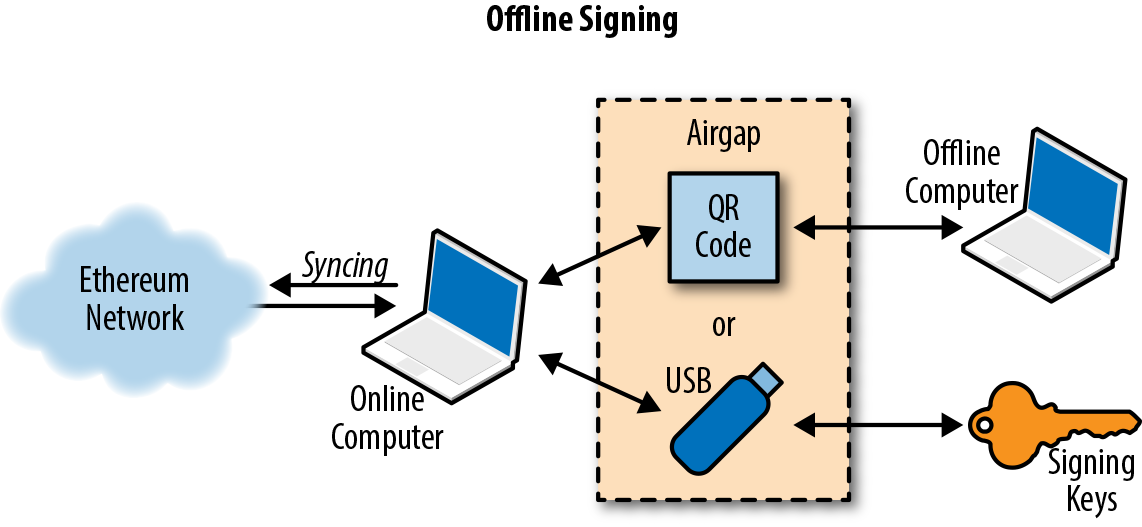
\includegraphics[width=1\columnwidth]{offline_signing} 
	\caption[Firma offline delle transazioni di Ethereum]{Firma offline delle transazioni di Ethereum}
	\label{fig:ofline_signing} 
\end{figure}

\section{Smart Contract}
Il termine smart contract è stato usato nel corso degli anni per descrivere un'ampia varietà di cose differenti. Nel contesto di Ethereum il termine in realtà è un po' improprio dato che gli smart contract Ethereum non sono né smart (intelligenti), né contract (legali). Tali contratti fanno piuttosto riferimento a programmi informatici immutabili che funzionano in modo deterministico in un contesto quale la macchina virtuale Ethereum (EVM) sul computer decentralizzato Ethereum. Ma vediamo questa affermazione per step:
\begin{description}
	\item[Programmi per computer] Gli smart contract sono semplicemente dei programmi per computer. La parola "contratto" non ha alcun significato legale per questo contesto.
	\item[Immutabile] Una volta implementato, il codice di un contratto non può essere cambiato, a differenza di un software tradizionale. Infatti l'unico modo per portare delle modifiche ad un proprio contatto è quello di ridistribuirne una nuova istanza.
	\item[Deterministico] L'esito di uno smart contract sarà lo stesso per tutti coloro che lo eseguiranno, dato il contesto della transazione e lo stato della blockchain Ethereum al momento di tale esecuzione.
	\item[Contesto EVM] Gli smart contract operano con un contesto di esecuzione limitato. Possono accedere al loro stato, al contesto della transazione che li ha richiamati e ad alcune informazioni sui blocchi più recenti.
	\item[Computer mondiale decentralizzato] L'EVM viene eseguita come istanza locale su ogni nodo Ethereum, ma poiché tutte le istanze di EVM operano sullo stesso stato iniziale e produrranno lo stesso stato finale, il sistema nel suo complesso opera come un singolo computer mondiale.
\end{description}
%
\subsection{Ciclo di vita di uno Smart Contract}
Gli smart contract sono solitamente scritti in un linguaggio di alto livello, come ad esempio Solidity. Per essere eseguiti nella EVM devono poi essere compilati in bytecode. Una volta compilati possono essere distribuiti sulla piattaforma Ethereum tramite la speciale transazione di creazione contratto che invia tale transazione all'indirizzo 0x0. Ogni contratto è identificato da un proprio indirizzo Ethereum che può essere utilizzato per l'invio di fondi o per richiamare le funzione in esso specificate. Diversamente dagli EOA, uno smart contract non ha associate delle chiavi. Tali contratti vengono eseguiti solamente se richiamati da una transazione. Un contratto può richiamare un altro contratto ma il primo della catena sarà per forza di cose richiamato da un qualche EOA. Nel caso in cui l'esecuzione dovesse fallire per un qualche motivo, termine gas o errore di qualche tipo, tutti i cambiamenti di stato avvenuti fino a quel momento vengono ripristinati a prima dell'esecuzione come se la transazione non fosse mai stata eseguita. Una transazione fallita viene comunque registrata come tentata, e l'etere speso a gas per l'esecuzione viene detratto dall'account di origine. 

Come accennato in precedenza, è importante ricordare che il codice di uno smart contract non può essere modificato. Tuttavia, un contratto può essere \textit{cancellato}, rimuovendo il codice e il suo stato interno, archiviazione, dal suo indirizzo, lasciando un account vuoto. Qualsiasi transazione inviata a quell'indirizzo dell'account dopo che il contratto è stato eliminato non comporta l'esecuzione di alcun codice, perché non esiste più alcun codice da eseguire. Per fare ciò si dovrà eseguire un apposito codice operativo chiamato SELFDESTRUCT. Tale operazione cosa una cifra in gas negativa, una sorta di rimborso del gas, questo per incentivare il rilascio di risorse. L'eliminazione di un contratto in questo modo non rimuove la cronologia delle transazioni del contratto, poiché la blockchain stessa è immutabile. La funzionalità SELFDESTRUCT sarà disponibile solamente se l'autore del contratto ha programmato il contratto per ottenere tale funzionalità, in caso contrario il contratto non potrà essere cancellato.

\subsection*{Linguaggi di alto livello per Ethereum}
L'EVM è una macchina virtuale che esegue una speciale forma di codice chiamata bytecode EVM, analoga alla CPU di un comune computer, che esegue codice macchina come x86\_64. E' possibile programmare i contratti Ethereum direttamente in bytecode, tuttavia la maggior parte dei programmatori preferisce ovviamente utilizzare un linguaggio di alto livello per poi convertire il codice prodotto in bytecode tramite un compilatore ad hoc. I linguaggi di programmazione possono essere classificati in due ampi paradigmi di programmazione: \textit{dichiarativo} e \textit{imperativo} , anche noti rispettivamente come \textit{funzionali} e \textit{procedurali}. Nella procedura dichiarativa, scriviamo funzioni che esprimono la logica di un programma, ma non il suo flusso. Viene utilizzata per creare programmi in cui non ci sono effetti collaterali, non ci saranno, infatti, combiamenti di stato al di fuori di una funzione. Haskel e SQL sono due di questi. Nella programmazione imperativa, al contrario, una procedura può cambiare sia la logica che il flusso di un programma. In questo contesto troviamo C++ e Java. Poi ci sono dei linguaggi di programmazione ibridi che incoraggiano la programmazione dichiarativa ma possono essere utilizzate anche per esprimere un paradigma di programmazione imperativo. Qui troviamo Lisp, JavaScript e Python. Qualsiasi linguaggio imperativo può essere usato per scrivere un paradigma dichiarativo. I linguaggi puramente dichiarativi, invece, non possono essere usati per scrivere un paradigma imperativo.

Mentre la programmazione imperativa è più comunemente utilizzata dai programmatori, può essere molto difficile scrivere programmi eseguiti esattamente come previsto. La capacità di qualsiasi parte del programma di cambiare lo stato di qualsiasi altro rende difficile ragionare sull'esecuzione di un programma e introduce molte opportunità per i bug. Nei contratti intelligenti, i bug costano letteralmente denaro e di conseguenza, è di fondamentale importanza scrivere contratti intelligenti senza effetti indesiderati. Per questo motivo, i linguaggi dichiarativi svolgono un ruolo molto più importante negli smart contract. Tuttavia, il linguaggio più utilizzato per i contratti intelligenti risulta Solidity che è imperativo.

\section{Solidity}
Solidity è stato creato dal Dr. Gavin Wood come linguaggio esplicito per scrivere smart contract per Ethereum. Il principale prodotto del progetto Solidity è il compilatore, \textit{solc}, che converte i programmi scritti in Solidity in linguaggio bytecode EVM. Ogni versione del compilatore corrisponde e compila una versione specifica di Solidity. Tale linguaggio segue un modello di versioning chiamato semantic versioning, che specifica la versione strutturandola in tre parti numeriche: MAJOR:MINOR:PATCH.

E' possibile installare il compilatore Solidity su Ubuntu / Debian seguendo le istruzioni riportate sull'apposita pagina http://olidity.readthedocs.io. Come già detto in precedenza ne esiste anche una versione web-based che include un IDE chiamato Remix, pensato per test iniziali e lo sviluppo di piccoli Smart Contract.

\subsection{Variabili e funzioni locali predefinite}
Quando un contratto viene eseguito nell'EVM, ha accesso ad un piccolo insieme di oggetti globali, tra cui \textit{block}, \textit{msg}, e \textit{tx}.
\begin{itemize}
	\item \textbf{msg} L'oggetto \textit{msg} contiene le informazioni del chiamante che può essere un EOA nel caso di una transazione, oppure una message call, nel caso la chiamata fosse originata da un altro contratto.
	\item \textbf{tx}  L'oggetto \textit{tx} fornisce un mezzo per accedere alle info relative alla transazione.
	\item \textbf{block}  L'oggetto \textit{block} contiene informazioni circa il blocco corrente.
	\item \textbf{address}  Qualsiasi indirizzo passato ha un numero di attributi e metodi richiamabili con il prefisso \textit{address}.
	\item \textbf{addmod, mulmod} per eseguire somme e moltiplicazioni in module.
	\item \textbf{keccak256, sha256, sha3, ripemd160} per calcolare l'hash del messaggio.
	\item \textbf{ecrecover} recupera l'indirizzo utilizzato per firmare il messaggio.
	\item \textbf{selfdestrunct} elimina il contratto inviando l'ether residuo.
	\item \textbf{this} si riferisce all'indirizzo dell'account attualmente in esecuzione.
\end{itemize}

\subsection{Funzioni di un contratto}
All'interno di un contratto possiamo definire delle funzioni richiamabili da una qualsiasi transazione EOA oppure da un altro contratto. La sintassi utilizzata per la scrittura di queste funzioni è la seguente:
%
\begin{lstlisting}
function FunctionName([parameters]) {public|private|internal|external}
	[pure|constant|view|payable] [modifiers] [returns (return types)]
\end{lstlisting}
%
\begin{table}[h]
	\centering
	\begin{tabular}{|c|p{10.5cm}|}
		\hline
		\lstinline|FuncionName| & identifica la funzione tramite un nome, utilizzato per richiamare tale funzione tramite transazioni EOA o da altri contratti.\\ \hline
		\lstinline|parameters| & specificano il tipo degli argomenti che devono essere passati alla finzione e il rispettivo nome che assumono all'interno di essa.\\ \hline
		\lstinline|public| & tali funzioni possono essere richiamate da altri contratti, o transazioni, o dall'interno del contratto che la implementa.\\ \hline
		\lstinline|external| & come le funzioni pubbliche ma non possono essere richiamate da procedure interne al contratto.\\ \hline
		\lstinline|internal| & sono accessibili solamente tramite procedure interne al contratto.\\ \hline
		\lstinline|private| & come le interne ma non sono richiamabili da contratti derivati.\\ \hline
		\lstinline|costant / view| & la funzione contrassegnata come view promette di non modificare lo stato, constant è un alias di view che sarà deprecato in futuro, il compilatore produrrà un warning in caso di utilizzo errato.\\ \hline
		\lstinline|pure| & tale funzione non legge ne scrive le variabili in memoria, opera solamente su argomenti e restituisce dati senza alcun riferimento a dai memorizzati.\\ \hline
		\lstinline|payable| & accetta pagamenti in entrata, se non implementata rifiutano tali transazioni. \\ \hline
	\end{tabular}
\end{table}
%
\subsection*{Considerazioni sul Gas}
Il gas è una risorsa limitata pensata per limitare la quantità massima di calcolo che Ethereum consentirà ad una trasazione di consumare. Se il limite di gas viene in qualche modo superato viene lanciata l'eccezione \lstinline|out of gas exception|, viene ripristinato lo stato dello smart contract a prima di tale esecuzione e tutto il gas speso fino a quel momento per tentare tale esecuzione viene speso come tassa di transazione e quindi non viene rimborsato. Il costo del gas può essere stimato tramite la seguente procedura:
\begin{lstlisting}
var contract = web3.eth.contract(abi).at(address);
var gasEstimate = contract.myMethod.estimateGas(arg1,arg2,{from: account});
\end{lstlisting}
\lstinline|gasEstimate| ci indicherà il numero di unità di gas necessarie per l'esecuzione del metodo \lstinline|myMethod|. Questa risulterà appunto una stima a causa della Turing completezza dell'EVM. Risulta infatti relativamente banale creare una funzione che richiederà quantità di gas molto diverse da quelle ritornate dalla sopracitata funzione. Per ottenere il prezzo del gas dalla rete e il relativo costo totale è possibile utilizzare:
\begin{lstlisting}
var gasPrice = web3.eth.getGasPrice();
var gasCostInEther = web3.fromWei((gasEstimate * gasPrice), 'ether');
\end{lstlisting}

\section{Sicurezza ed attacchi agli Smart Contract}
La sicurezza è una delle considerazioni più importanti quando si procede con la scrittura degli Smart Contract dato che gli errori sono costosi e facilmente sfruttabili. In questa sezione andiamo a esaminare le best practice di sicurezza e quali sono le pratiche che possono indurre vulnerabilità all'interno dei nostri contratti.
La programmazione difensiva risulta lo stile di sviluppo che più si adatta agli smart contract. Ma andiamo ad elencare quali sono le migliori tecniche:
\begin{description}
	\item[Minimalismo] La complessità risulta essere nemica della sicurezza. Più semplice è il codice più facile risulterà individuare bug o comportamenti imprevisti. 
	\item[Riutilizzo del codice] Cerca di non reinventare la ruota. Se esiste già una libreria o un altro contratto che fa già ciò che intendi implementare, riutilizzalo. Se più procedure vengono ripetute più volte all'interno del proprio codice, valutare se creare una funzione che implementi tale procedura.
	\item[Qualità del codice] Il codice degli smart contract non perdona, ogni bug o funzionamento inaspettato può portare ad una perdita monetaria.
	\item[Leggibilità] Il codice deve essere chiaro e facile da comprendere. I contratti sono pubblici e chiunque può accedere al bytecode ed eseguire il reverse engineering. Pertanto è consigliabile sviluppare il proprio lavoro in modo pubblico, utilizzando metodologie collaborative e open source.
	\item[Test coverage] Metti alla prova tutto ciò che puoi. Gli smart contract vengono eseguiti in un ambiente pubblico e chiunque può testare qualsiasi contratto con qualsiasi input.
\end{description}
Gli effettivi rischi per la sicurezza che espongono i propri contratti a potenziali attacchi. Vediamone alcuni:
\subsection*{Reentracy}
Una delle caratteristiche principali degli smart contract Ethereum è la loro capacità di richiamare e quindi utilizzare codice all'interno di altri contratti. I contratti, di base, gestiscono anche dell'ether che può essere inviato ad altri indirizzi. Questa operazione richiede che un contratto abbia la capacità di inviare chiamate verso l'esterno che possono essere dirottate da eventuali aggressori che possono quindi forzare i contratti ad eseguire ulteriore codice, tramite una funzione di fallback. Un attacco di questo tipo fu utilizzato nel famigerato attacco DAO. Per prevenire questo tipo di attacco è possibile ricorrere a delle contromisure. Possiamo infatti utilizzare una funzione di trasferimento integrata che consente di inviare solamente 2300 unità di gas per un'invocazione esterna. Questa cifra non sarà sufficiente per coprire il costo di un'eventuale ulteriore invocazione da parte del contratto chiamato.

\subsection*{Arithmetic Over / Underflows}
Una macchina virtuale Ethereum specifica i tipi di dati a dimensione fissa pr i numeri interi. Ciò significa che una variabile intera può rappresentare solo un certo intervallo di numeri. Un \lstinline|uint8| può rappresentare solamente numeri nell'intervallo [0-255]. Se si tentasse di rappresentare il numero 256 all'interno di un \lstinline|uint8| il numero risultante sarà 0. Se quindi non si presta la dovuta attenzione alcune operazioni possono generare dei risultati inaspettati. L'attuale tecnica convenzionale per proteggersi da vulnerabilità di over / underflow consiste nell'utilizzare o costruire librerie matematiche che sostituiscono gli operatori matematici standard quali addizione, sottrazione e moltiplicazione (la divisione è esclusa in quanto non causa over / underflow e l'EVM ritorna alla divisione di 0).

\subsection*{Delegate Call}
Gli opcode \lstinline|CALL| e \lstinline|DELEGATECALL| sono utili agli sviluppatori per modulare il loro codice. Le message call a contratti esterni sono gestita dalle \lstinline|CALL|, in base al quale il codice viene eseguito nel contesto del contratto / funzione. L'opcode \lstinline|DELEGATECALL| risulta simile se non per il fatto che il codice viene eseguito nel contesto del contratto chiamato e \lstinline|msg.sender| e \lstinline|msg.value| rimangono invariati. Questa funzione permette di implementare librerie, consentendo agli sviluppatori di distribuire il codice rendendolo utilizzabile in contratti futuri. Come risultato della conservazione del contesto di \lstinline|DELEGATECALL|, la creazione di librerie personalizzate prive di vulnerabilità non è così semplice come si potrebbe pensare. Il codice nelle librerie stesse può essere sicuro e privo di punti deboli, tuttavia, quando viene eseguito nel contesto di un'altra applicazione, possono verificarsi nuove vulnerabilità. Come regola generale, quando si utilizza \lstinline|DELEGATECALL| prestare attenzione al possibile contesto di chiamata sia del contratto di libreria che del contratto di chiamata e, quando possibile, creare librerie senza stato.

\subsection*{Default Visibilities}
Le funzioni in Solidity presentano delle specifiche di visibilità che determinano se una funzione può essere richiamata esternamente da altri utenti / contratti oppure solo internamente / esternamente. Come visto in precedenza esistono quattro specifiche di visibilità, tra queste \lstinline|public| risulta la proprietà predefinita nel caso in cui non ne venga indicata un'altra. Questo fa si che, se non si porta la dovuta attenzione, alcune funzioni con determinati scopipotrebbero essere richiamabili anche dall'esterno deviando il comportamento standard atteso del contratto. È buona norma specificare sempre la visibilità di tutte le funzioni in un contratto, anche se intenzionalmente \lstinline|public|.

\subsection*{Entropy Illusion}
Tutte le transazioni su Ethereum sono delle operazioni sullo stato eseguite in modo deterministico. Ciò significa che ogni transazione modifica lo stato globale dell'ecosistema Ethereum in modo calcolabile. Ciò implica che all'interno di Ethereum non ci può essere alcuna fonte di entropia o casualità. Raggiungere l'entropia decentralizzata è un problema ben noto per il quale sono state proposte molte soluzioni, tra cui \textit{RANDAO} , o l'utilizzo di una catena di hash. Se si intende sviluppare dei contratti per il supporto ad applicazioni che necessitano di una ottima fonte di casualità si deve trovare una soluzione per implementarla. Questo ci porta a concludere che la funte di casualità deve provenire dall'esterno della blockchain.

\subsection*{Denial of Service (DoS)}
Questa categoria è molto ampia, ma fondamentalmente consiste in attacchi in cui gli utenti possono rendere inoperabile un contratto per un periodo di tempo, o in alcuni casi in modo permanente. Questo può intrappolare etere in questi contratti per sempre. Esistono vari modi in cui un contratto può diventare inutilizzabile, vediamone alcuni:
\begin{itemize}
	\item \textbf{Looping attraverso mappature o array manipolati esternamente} Questo schema si verifica in genere quando un proprietario desidera distribuire token a degli investitori con una tecnica dinamica. In linea di principio un malintenzionato può creare $n$ account ed utilizzarli aggiungendoli ad una potenziale lista di account candidabili ad una vincita. Ciò può essere fatto in modo tale che il gas necessario per eseguire il ciclo \lstinline|fot| superi il limite del gas di blocco, rendendo funzione non più eseguibile.
	\item \textbf{Owner operations} Un altro schema comune appare quando il passaggio allo stato successivo è vincolato dal consenso del proprietario dello smart contract. Un esempio potrebbe essere un contratto Initial Coin Offering (ICO):
	\begin{lstlisting}
	bool  public isFinalized = false;
	addres public owner;
	
	function finalize () public {
		require (msg.sender == owner);	■\label{row:transfer-require}■
		isFinalized = true ;
	}
	
	// ... extra ICO functionality
	
	function transfer(address _to, uint _value) returns (bool) {
		require(isFinalized);
		super.transfer(_to,_value)
	} 
	\end{lstlisting}
	In questi casi, se l'utente privilegiato perde le proprie chiavi private o diventa inattivo, l'intero contratto token diventa inutilizzabile.
	
	\item \textbf{Avanzamento basato su chiamate esterne} A volte i contratti vengono scritti in modo tale che passare a un nuovo stato richiede l'invio di etere a un indirizzo o l'attesa di qualche input da una fonte esterna. Questi modelli possono portare a attacchi DoS quando la chiamata esterna non riesce o viene impedita per ragioni esterne.
\end{itemize}
Una delle tecniche preventive, specie per le owner operations, sta nel evitare che le istruzioni di blocco siano dipendenti solamente da invocazioni che provengono dall'account del creatore. Nell'esempio sopra riportato si potrebbe pensare di riscrivere l'istruzione di \lstinline|require| alla riga~\ref{row:transfer-require} facendola dipendere anche da un fattore di tempo, per esempio \lstinline!require(msg.sender == owner || now > unlockTime)!. In questo modo, nel caso in cui il creatore del contratto non richiami la funzione \lstinline|finalize()|, o fosse impossibilitato a farlo, chiunque può eseguire il cambio di stato a patto che sia passato un tempo \lstinline|unlockTime|, sbloccando così i fondi altrimenti bloccati.

\subsection*{Autenticazione tramite \lstinline|tx.origin|}
Solidity ha una variabile globale \lstinline|tx.origin|, che contiene l'indirizzo di chi ha originariamente invito la chiamata o transazione. L'utilizzo improprio di questa variabile rende un contratto vulnerabile ad una attacco simile al phishing. Supponiamo di trovare un contratto che dispensa ether tramite la funzione \lstinline|withdrawAll| sse \lstinline|tx.origin == owner|. 
\begin{lstlisting}
	function withdrawAll (indirizzo  _recipient) public {
		require (tx.origin  == owner);
		_recipient.transfer (this.balance);
	}
\end{lstlisting}
Creiamo ora un nuovo contratto ad hoc che richiama la funzione \lstinline|withdrawAll|, all'interno del contratto vittima, passando come indirizzo \lstinline|_recipient|, l'indirizzo dell'attaccante. Se la funzione di questo nuovo contratto viene invocata dal proprietario del primo contratto, richiamerà la funzione \lstinline|withdrawAll| della vittima che trasferirà i fondi all'account dell'attaccante. Questo non significa che la variabile \lstinline|tx.origin| non debba essere utilizzata, ma piuttosto deve essere utilizzata con cautela e non per autorizzare operazioni importanti. 

\section{Oracoli}
Gli oracoli sono sistemi in grado di fornire fonti di dati esterne agli smart contract di Ethereum, idealmente sono dei Sistemi \textit{trustless}, senza fiducia, nel senso che non hanno bisogno di essere fidati perché operano su principi decentrati. Un componente chiave della piattaforma Ethereum è la macchina virtuale Ethereum, con la sua capacità di eseguire programmi e aggiornare lo stato di Ethereum, vincolato da regole di consenso, su qualsiasi nodo della rete decentralizzata. Al fine di mantenere un consenso, l'esecuzione dell'EVM deve essere totalmente deterministica e basata unicamente sul contesto condiviso dello stato di Ethereum e delle transazioni firmate. Tutto ciò porta a due conseguenze principali:
\begin{enumerate}
	\item non ci può essere una fonte intrinseca di casualità per l'EVM e per gli smart contract con cui lavorare;
	\item i dati estrinseci possono essere introdotti solo come il carico utile di dati di una transazione.
\end{enumerate}
In particolare, in un sistema come Ethereum, non può esistere una una funzione casuale perché porterebbe ad un effetto disastroso. Una funzione puramente casuale porta infatti a risultati diversi ad ogni sua esecuzione. Questo non deve essere possibile in Ethereum altrimenti due nodi diversi che eseguono lo stesso contratto arriverebbero a due conclusioni differenti nonostante entrambi nodi abbiano eseguito lo stesso codice nel medesimo contesto. Come tale non ci sarebbe modo per la rete di arrivare ad un consenso decentrato. Si noti che le funzioni pseudo casuali, come le funzioni hash, crittograficamente sicure, non sono sufficienti per molte applicazioni, vedi per esempio il gioco d'azzardo, che simula lanci di monete per risolvere i pagamenti delle scommesse. Un minatore può infatti ottenere un vantaggio includendo nei blocchi solo le transazioni per le quali vincerà. Usiamo gli oracoli per tentare di risolvere questa tipologia di problemi. Gli oracoli forniscono un modo trustless di ottenere informazioni estrinseche\footnote{Informazioni fuori dalla Blockchain.} sulla piattaforma Ethereum per gli Smart Contract. Gli oracoli possono quindi essere considerati un meccanismo per colmare il divario tra il mondo fuori catena e i contratti intelligenti. Consentendo ai contratti intelligenti di far rispettare le relazioni contrattuali basate su eventi e dati del mondo reale. Alcuni oracoli forniscono dati che sono specifici di una determinata fonte di dati privata. La fonte di tali dati deve essere pienamente affidabile. E' possibile progettare un Oracle client implementato in  Solidity che per definizione dovranno implementare alcune funzioni chiave, includendo la possibilità di:
\begin{itemize}
	\item Raccogliere i dati da una fonte off-chain.
	\item Trasferire i dati sulla catena tramite un messaggio firmato.
	\item Rendere i dati disponibili in memoria all'interno di uno smart contract.
\end{itemize}
Una volta che i dati sono disponibili in memoria in un contratto intelligente, è possibile accedervi tramite altri smart contract tramite chiamate di messaggi che invocano una funzione di "recupero" del contratto intelligente dell'oracolo.

\subsection*{Autenticazione dei dati}
Se supponiamo che la fonte dei dati interrogati da un DApp sia autorevole e affidabile, dobbiamo essere in grado di fidarci di questo meccanismo dal momento in cui esiste la possibilità che i dati possono essere manipolati durante il transito. Dobbiamo quindi essere in grado di testare l'integrità dei dati restituiti. Esistono due approcci comuni per l'autenticazione: \textit{authenticity proofs} e \textit{trusted execution environments} (TEE). Le authenticity proofs, o prova di autenticità, sono garanzie crittografiche che i dati non sono stati manomessi.  Oraclize è un esempio di servizio oracolo che sfrutta una varietà di prove di autenticità. Una prova di questo tipo attualmente disponibile per le query di dati dalla rete principale di Ethereum è la prova TLSNotary. Le prove TLSNotary consentono a un client di fornire prove ad una terza parte, che il traffico Web HTTPS sia verificato tra il client-server.
Oltre agli oracoli nel contesto della richiesta e consegna di dati, esiste anche la possibilità di utilizzarli per eseguire calcoli arbitrari. Anzichè limitarsi a trasmettere risultati di una query , è possibile utilizzare gli oracoli per eseguire calcoli su un insieme di input e restituire un risultato che altrimenti potrebbe essere stato impossibile calcolare sulla catena.
Possono essere implementati dei contratti che tengono traccia del valore di cambio valuta, per esempio ETH/USD che sonderà continuamente il prezzo ETH/USD da un'API e archivierà il risultato, rendendolo così utilizzabile.

\subsubsection{Conclusioni}
Come abbiamo visto gli oracoli forniscono un servizio cruciale per gli smart contract, portando fatti esterni all'interno dell'escuzione del contratto. Tutto ciò introducendo comunque un rischio significativo: se le fonti sono attendibili e possono essere compromesse potrebbero portare ad un'esecuzione inaspettata degli smart contract che alimentano. Si dovrà quindi prestare molta attenzione al modelle di fiducia che si adotta. Gli oracoli decentrati possono risolvere alcune di queste preoccupazioni e offrire contratti intelligenti di Ethereum senza dati esterni. 

\section{Applicazioni decentralizzate (\DH App)}
Fin dai primi giorni i fondatori di Ethereum avevano una visione molto più ampia che andava oltre gli smart contract. L'idea di fondo era reinventare il web creandone uno nuovo dal nome \textit{web3}. I contratti intelligenti, di cui abbiamo parlato fin qui, sono un modo per decentrare la logica di controllo e le funzioni di pagamento delle applicazioni. Web3 \DH App riguarda la decentralizzazione di tutti gli altri aspetti di un'applicazione: archiviazione, messaggistica, naming ecc\dots
%
\begin{figure}
\centering 
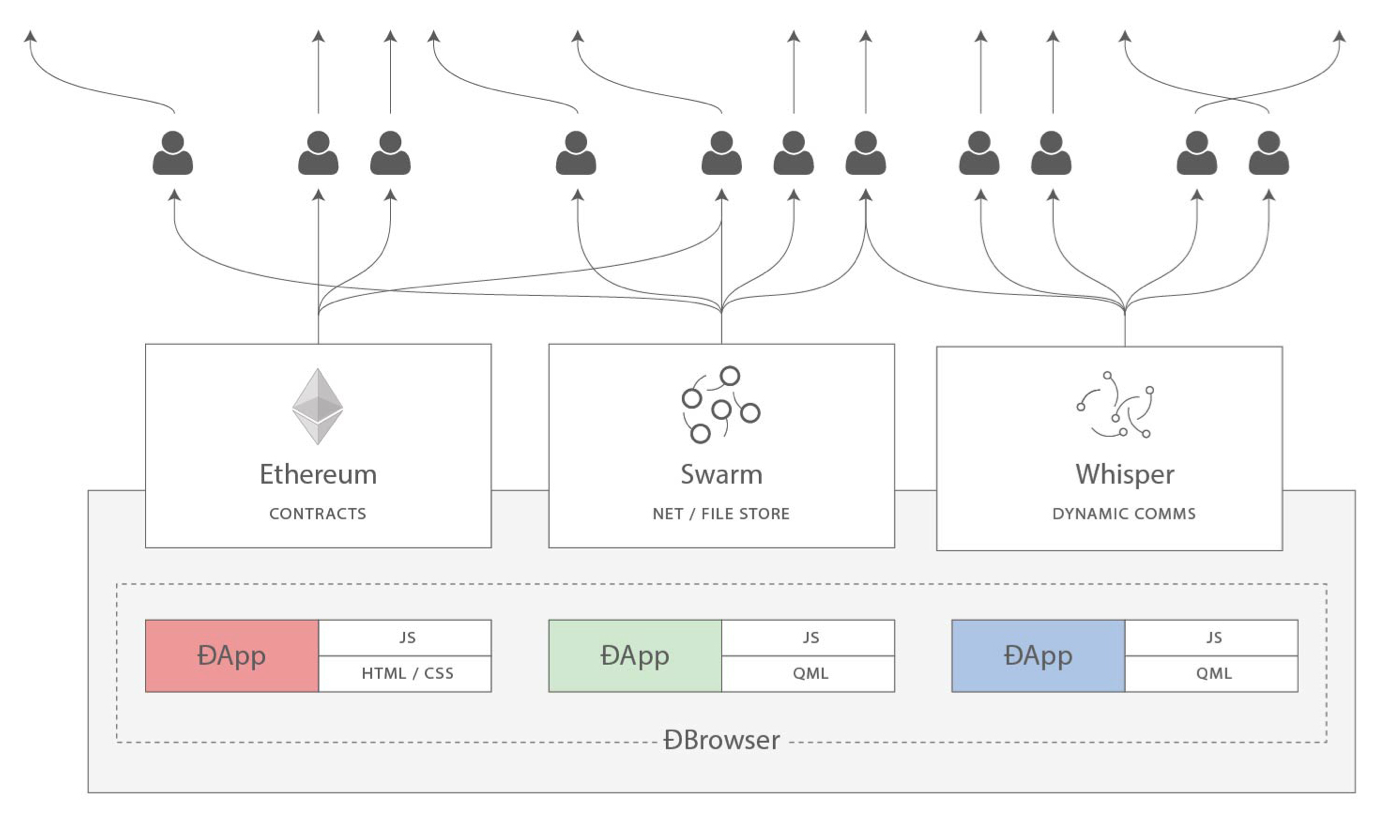
\includegraphics[width=1\columnwidth]{web3suite} 
\caption[Web3 web decentralizzato che utilizza smart contract e tecniche P2P]{Web3 web decentralizzato che utilizza smart contract e tecniche P2P}
\label{fig:web3siute} 
\end{figure}
%
Una \DH App è quindi un'applicazione per lo più, o interamente decentralizzata nei suoi vari aspetti: Software di back-end e frontend, archiviazione dati, comunicazioni messaggi e risoluzione dei nomi. Ognuno di questi può essere alquanto centralizzato o piuttosto decentralizzato. Ci sono diversi vantaggi che può portare una architettura decentralizzata di questo tipo:
\begin{itemize}
	\item \textbf{Elasticità:} la logica di business è controllata da uno smart contract, la back-end di una \DH App sarà completamente distribuita e gestita su blockchain, non sarà quindi vittima di possibili tempi di inattività.
	\item \textbf{Trasparenza:} la natura on-chain consente a tutti di visionare il codice delle varie funzioni.
	\item \textbf{Resistenza alla censura:} finchè un utente avrà accesso alla rete Ethereum sarà sempre in grado di interagire con una \DH App senza dipendere da nessun controllo centrale o qualsiasi fornitore di servizi.
\end{itemize}
Ma vediamo in dettaglio i vari aspetti di un'applicazione decentralizzata:

\subsubsection{Back-end (Smart Contract)}
Nelle \DH App, per archiviare la logica aziendale, si fa utilizzo degli smart contract sarà quindi così anche per lo stato di tale app. Possiamo pensare allo smart contract come quella componente che va a sostituire la back-end di un server in una normale applicazione. Da notare però che qualsiasi operazione eseguita con un contratto risulterà molto costosa per questo motivo si dovrà mantenere tale logica il puù minimale possibile e  soprattutto identificare quali aspetti della \DH App richiedono un'esecuzione affidabile e decentralizzata. Una considerazione importante di cui tener conto quando si procede con l'implementazione di uno smart contract è l'incapacità di modificare il codice una volta implementato. Può essere cancellato ma solamente se è stato programmato il codice operativo \lstinline|SELFDESTRUCT|. Ultima importante considerazione riguarda il design dell'architettura di uno smart contract. Un contratto monolitico molto grande può costare molto gas una volta eseguito. Si può scegliere di diminuire il carico integrando calcoli provenientri da fonti off-chain, ma questo significa che qualsiasi utilizzatore di questo servizio si drovrà fidare di tali fonti esterne.

\subsubsection{Frontend (Web User Interface)}
A differenza della logica di business di \DH App, che richiede di comprendere l'EVM e nuovi linguaggi come ad esempio Solidity, l'interfaccia lato client di una \DH App può utilizzare tecnologie web standard come HTML, CSS, JavaScript, ecc. Ciò consente quindi ad uno sviluppatore web tradizionale di utilizzare strumenti, librerie e framework famigliari. Le interazioni con Ethereum, come la firma di messaggi, l'invio di transazioni e la gestione di chiavi, sono spesso condotte attraverso il browser web, tramite un'estensione come MetaMask. Il frontend è in genere collegato a Ethereum tramite la libreria JavaScript \textit{web3.js}. 

\subsubsection{Data Storage}
A causa degli elevati costi del gas e del limite di gas a blocchi attualmente basso, i contratti intelligenti non sono adatti per archiviare o elaborare grandi quantità di dati. Pertanto, la maggior parte dei DApp utilizza servizi di archiviazione dati fuori catena, il che significa che memorizzano i dati ingombranti dalla catena Ethereum, su una piattaforma di archiviazione dati. La piattaforma di archiviazione dati può essere centralizzata (ad esempio, un tipico database cloud), oppure i dati possono essere decentralizzati, archiviati su una piattaforma P2P come l'IPFS o la piattaforma Swarm di Ethereum.
Lo storage P2P decentralizzato è ideale per archiviare e distribuire asset statici di grandi dimensioni come immagini, video e le risorse dell'interfaccia Web frontend dell'applicazione.

\subsubsection{Inter-Planetary File System (IPFS)}
E' un sistema decentralizzato per content-addressable per la distribuzione di oggetti memorizzati su di una rete P2P. "Content-addressable" significa che di ogni contenuto viene eseguito l'hash e questo hash verrà utilizzato per identificare tale file. Sarà così possibile recuperare qualsiasi file da qualsiasi nofo IPFS tramite il suo hash. IPFD mira a sostituire HTTP come protocollo per la consegna di applicazioni web.

\subsubsection{Swarm}
E' un altro sistema di archiviazione content-addressable simile a IPFS. Swarm è stato crato dalla Ethereum Fondation come parte della suite Go-Ethereum. Come IPFS, consente di archiviare file che vengono diffusi e reppliacti sui nodi Swarm. Il riferimento ai vari files viene eseguito sempre tramite hash e consente di accedere a un sito Web da un sistema P2P decentralizzato, anziché da un server Web centrale.

\subsubsection{Whisper}
Un altro componente importante di una qualsiasi applicazione è la comunicazione tra processi, il poter scambiare, quindi, messaggi tra applicazioni, diverse istanze dell'applicazione o tra i suoi vari utenti. Solitamente questo si ottiene facendo riferimento ad un server centrale, tuttavia esistono una varietà di alternative decentralizzate che offrono messaggistica su di una rete P2P. Il più importante protocollo di messaggistica P2P per \DH App risulta essere Whisper, che fa anche lui parte della suite Go-Ethereum.

\subsubsection{Ethereum Name Service (ENS)}
E' possibile progettare il miglior smart contract al mondo ma se non si fornisce una buona interfaccia per gli utenti, questi non saranno in grado di accedervi e quindi fruire del servizio. Su internet tradizionale, il Domani-Name-Sever (DNS) ci consente di navigare utilizzando dei nomi comprensibili all'uomo, mentre risolviamo quei nomi in indirizzi IP, recuperando così i contenuti cercati. Sulla blockchain Ethereum, l'Ethereum Naming System (ENS) risolve lo stesso problema, ma in modo decentralizzato. ENS è più di uno smart contract, è un \DH App fondamentale in sé, che offre un servizio di nomi decentralizzato. Inoltre, ENS è supportato da svariate \DH Apps per la registrazione e la gestione delle aste dei nomi registrati. ENS dimostra come le \DH App possono lavorare insieme. 

\section{La macchina virtuale di Ethereum}
Il cuore del protocollo Ethereum è appunto l'Ethereum Virtual Machine o EVM in breve. Come is può intuire da nome, si tratta di un motore di calcolo non molto diverso dalle macchine virtuali per il framework Microsoft .NET o di altri linguaggi compilati in bytecode come Java. Più in dettaglio, l'EVM è la parte di Ethereum che gestisce la distribuzione e l'esecuzione di contratti intelligenti. Le semplici transazioni di valore tra due EOA non devono coinvolgerlo ma si dovrà occupare di tutto ciò che comporta un aggiornamento di stato. L'EVM Ethereum può essere concepito come un computer decentralizzato globale contenente milioni di oggetti eseguibili, ciascuno con un proprio archivio di dati permanente. 
%
\begin{figure}
	\centering 
	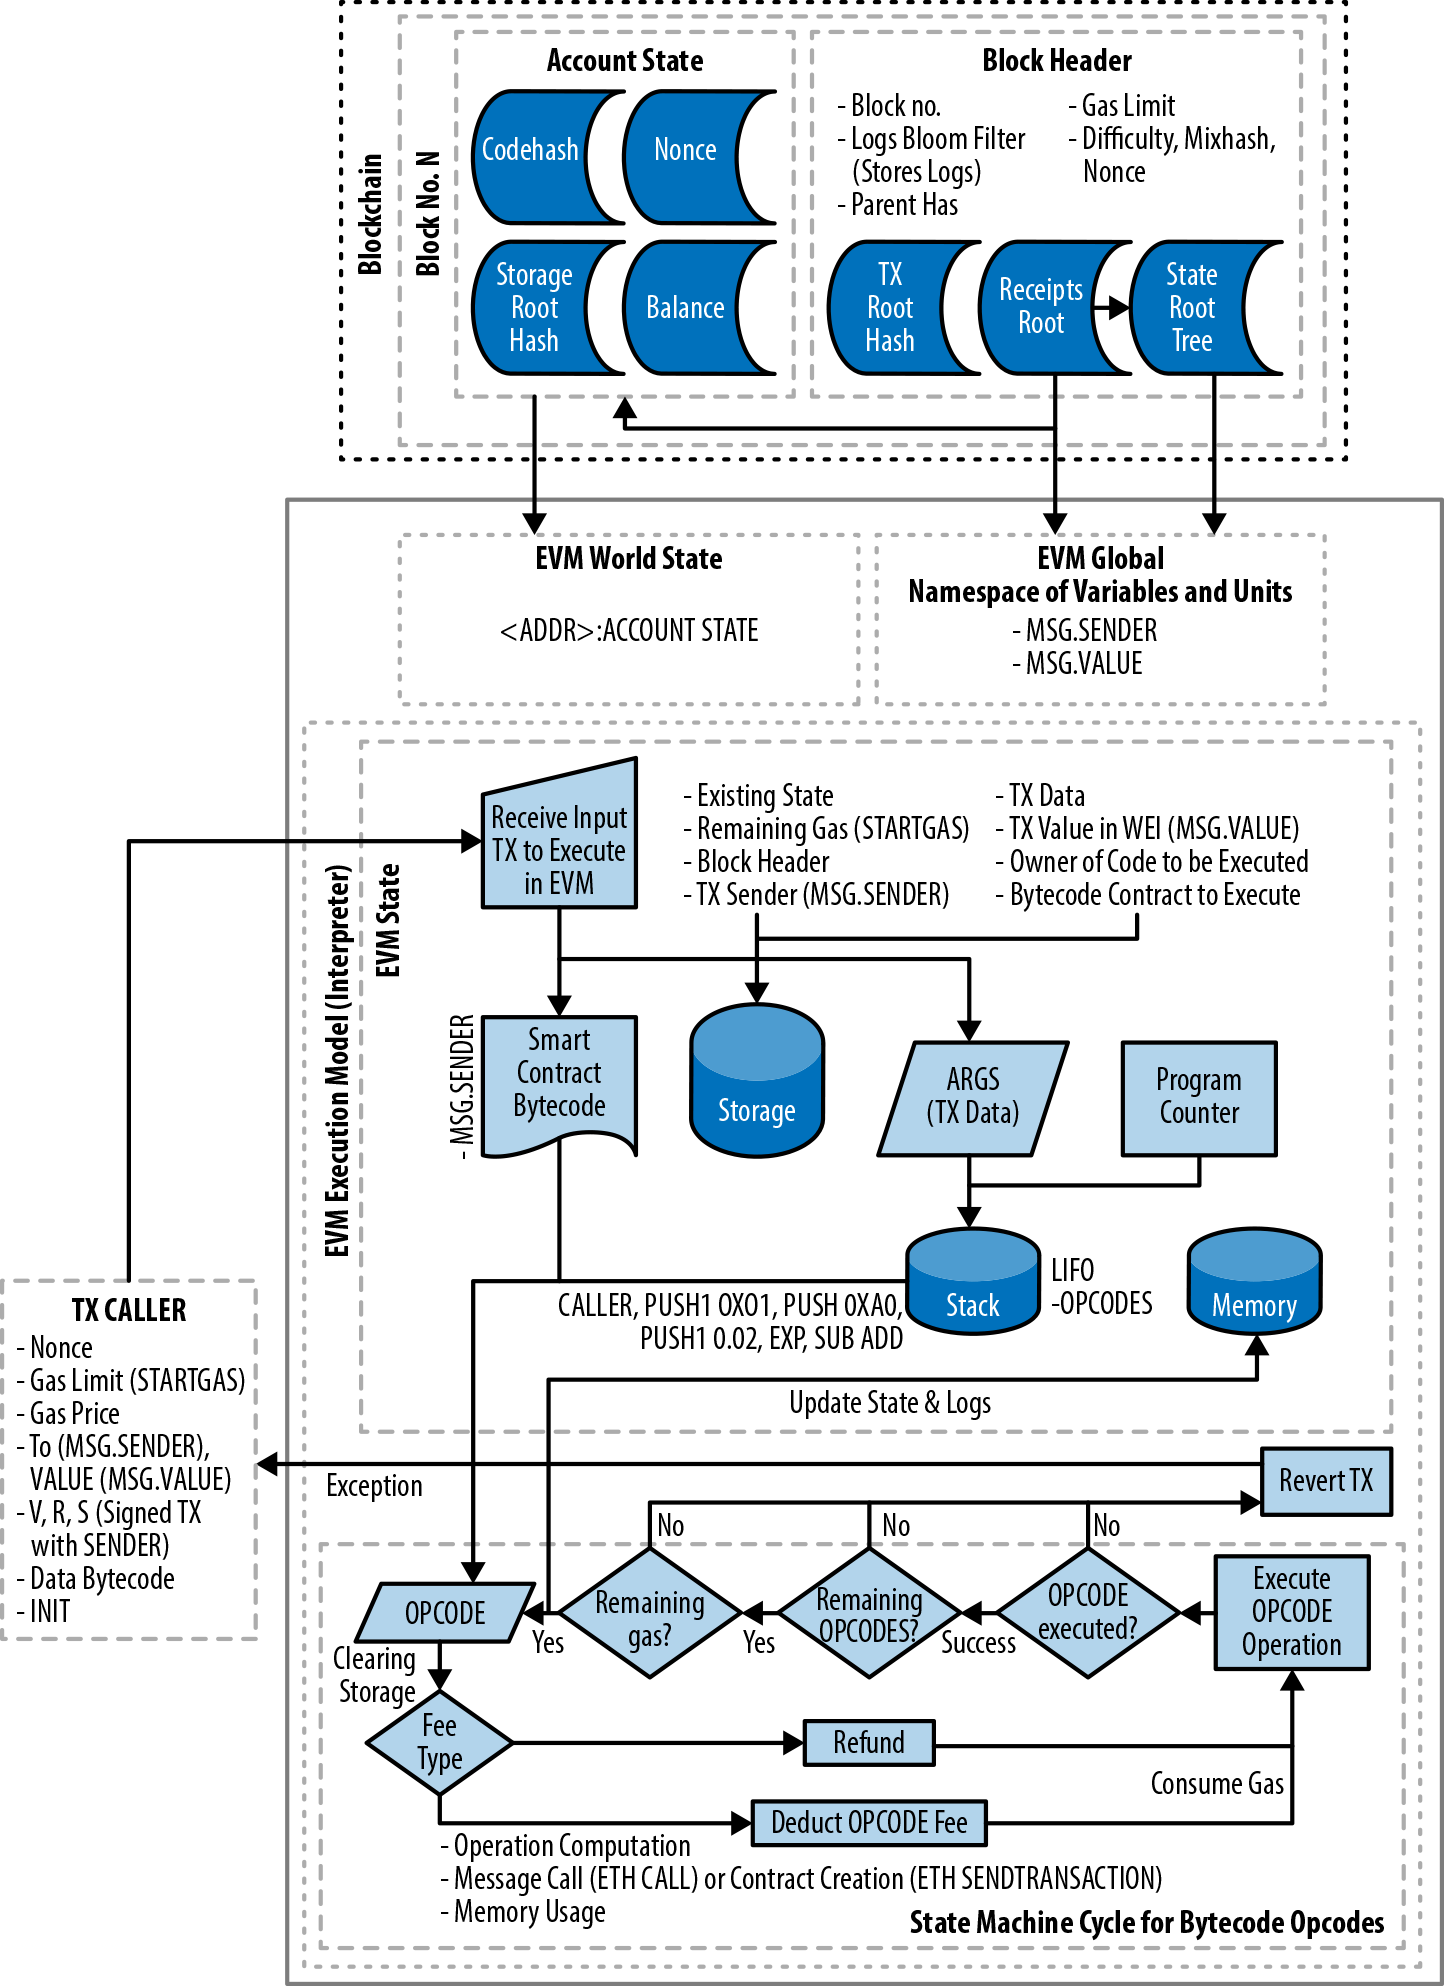
\includegraphics[width=1\columnwidth]{evm-architecture} 
	\caption[Architettura dell'EVM]{Architettura e contesto dell'EVM.}
	\label{fig:evm-architecture} 
\end{figure}
%
L'EVM è una macchina di Turing quasi completa, "quasi" perché tutti i processi in esecuzione sono limitati ad una numero finito di passaggi computazionali in base alla quantità di gas disponibile per ogni esecuzione, questo per garantire la terminazione di un qualsiasi codice sottoposto. L'architettura dell'EVM è basata su stack nel quale vengono salvati tutti i valori in memoria, ha diversi componenti di dati utilizzati:
\begin{itemize}
	\item La ROM di codice di programma immutabile, caricata con il bytecode del contratto intelligente da eseguire.
	\item Una memoria volatile, con ogni posizione esplicitamente inizializzata a zero.
	\item Una memoria permanente che fa parte dello stato di Ethereum, anch'essa inizializzata a zero.
\end{itemize}
Uno schema più completo lo si può vedere in Figura~\ref{fig:evm-architecture}.

\subsection*{Contronto con la tecnologia esistente}
Il termine "macchina virtuale" viene spesso applicato alla virtualizzazione di un computer reale, in genere da un "hypervisor" come VirtualBox o QEMU o da un'intera istanza del sistema operativo, come KVM di Linux. Questi devono fornire un'astrazione software dell'hardware effettivo, delle chiamate di sistema e altre funzionalità del kernel. EVM opera in un dominio molto più limitato: è solo un motore di calcolo e, in quanto tale, fornisce un'astrazione di solo computazione e archiviazione, simile, ad esempio, alle specifiche Java Virtual Machine (JVM). Da un punto di vista di alto livello, la JVM è progettata per fornire un ambiente di runtime che è indipendente dal sistema operativo o hardware host sottostante, consentendo la compatibilità su un'ampia varietà di sistemi. Linguaggi di programmazione di alto livello come Java o Scala (che usano JVM) o C\# (che usa .NET) sono compilati nel set di istruzioni bytecode della rispettiva macchina virtuale. Allo stesso modo, EVM esegue il proprio set di istruzioni bytecode, in cui vengono compilati i linguaggi di programmazione come LLL, Serpent, Mutan o Solidity.

\subsubsection{Stato di Ethereum}
Il compito dell'EVM è di aggiornare lo stato di Ethereum calcolando transizioni di stato valide come risultato dell'esecuzione del codice dello smart contract, come definito dal protocollo Ethereum. Quando una transazione richiama una funzione di un ceto smart contract, viene creata una EVM con tutte le informazioni richieste in relazione al blocco corrente a alla specifica transazione in elaborazione. In particolare l'EVM viene caricata con il codice del contratto chiamato, il program counter impostato a zero, lo storage locale viene caricato dallo storage dell'account di tale contratto, la memoria invece viene azzerata. Una variabile di particolare importanza è la fornitura di gas per l'esecuzione corrente, impostata sulla quantità di gas pagata dal mittente all'inizio della transazione. Mentre l'esecuzione del codice avanza, l'erogazione del gas viene ridotta in base al costo di ogni singola operazione eseguita. Se in qualsiasi momento venisse esaurito il gas, verrà lanciata l'eccezione Out-Of-Gas causando l'interruzione immediata dell'esecuzione e la transazione viene interrotta. Non vengono apportate modifiche allo stato precedente ad eccezione del nonce del mittente che viene incrementato, il gas speso per l'esecuzione fino all'interruzione non viene rimborsato e va a pagare il beneficiario del blocco per le risorse utilizzate fino al punto d'arresto. Tuttavia, se l'esecuzione viene completata correttamente, lo stato viene aggiornato per corrispondere alla versione dell'EVM in quel momento. 

\subsubsection{Turing completezza e Gas}
Come abbiamo già accennato, in termini semplici, un sistema o un linguaggio di programmazione è Turing completo se può eseguire qualsiasi programma. Un aspetto importante è che non possiamo dire, a priori, semplicemente guardando un programma, se tale programma terminerà o meno. Dobbiamo per forza procedere con l'esecuzione del programma ed attendere la sua terminazione per scoprirlo. Una delle possibilità è che il programma in questione non termini e questo ci porterebbe, in caso lo eseguissimo, ad attendere un tempo infinito. Questo si chiama halting problem, e sarebbe un grosso problema per Ethereum se non fosse affrontato. Se l'EVM eseguisse un programma di questo tipo diventerebbe inutilizzabile. Tuttavia, tramite l'utilizzo del Gas, c'è una soluzione: se dopo l'esecuzione di una quantità massima di calcolo , l'esecuzione non è terminata, tale procedura viene interrotta dall'EVM. Ciò rende l'EVM una macchina di Turing quasi completa dato che può eseguire qualsiasi programma inserito in essa, ma solo se termina entro una determinata quantità di calcolo. Questo limite non è fisso in Ethereum: puoi pagare per aumentarlo al massimo, chiamato il "limite del gas di blocco", e tutti possono concordare di aumentarlo nel tempo. 

\subsection*{Gas}
È l'unità di Ethereum per misurare le risorse computazionali e di archiviazione necessarie per eseguire azioni sulla blockchain di Ethereum. Diversamente da Bitcoin, le cui commissioni di transazione tengono conto solo delle dimensioni di una transazione in kilobyte, Ethereum deve tenere conto di ogni passo di calcolo eseguito dalle transazioni e dell'esecuzione del codice dello smart contract richiamato. ogni operazione eseguita da una transazione o contratto costa una quantità fissa di gas, vediamo alcuni esempi presi dal Yellow Paper di Ethereum:
\begin{itemize}
	\item La somma di due numeri costa 3 gas.
	\item Il calcolo di un hash Keccak-256 costa 30 gas + 6 gas per ogni 256 bit di dati sottoposti a hash.
	\item L'invio di una transazione costa 21.000 gas.
\end{itemize}
Prima di ogni operazione, l'EVM verifica che vi sia abbastanza gas da pagare per l'esecuzione dell'operazione. Se non c'è abbastanza gas, l'esecuzione viene interrotta e la transazione viene ripristinata. Se, invece, l'EVM raggiunge la fine dell'esecuzione con successo, senza esaurire il gas, il costo del gas utilizzato viene pagato al minatore come commissione di transazione, convertito in etere in base al prezzo del gas specificato nella transazione:
%
\begin{align*}
commissione Minatore &= costo Gas * prezzo Gas\\
gas Rimanente &= limite Gas - costo Gas\\
etere Rimborsato &= prezzo Rimanente Gas * Gas 
\end{align*}

\subsubsection{Costo del gas e prezzo del gas}
Mentre il conto del gas è misurato in base allo sforzo computazionale e di storage dell'EVM Ethereum, anche il gas stesso ha un prezzo in ether. Quando si esegue una transazione, il mittente specifica il prezzo del gas che è disposto a pagare (in etere) per ogni unità di gas, consentendo al mercato di decidere la relazione tra il prezzo dell'etere e il costo delle operazioni di calcolo (misurato in gas) :
%
\[ commissione Di Transazione = gas Totale Utilizzato * prezzo Gas Pagato \]
%
Quando si costruisce un nuovo blocco, i minatori della rete Ethereum possono scegliere tra le transazioni in sospeso selezionando quelle che offrono di pagare un prezzo del gas più alto. Offrire un prezzo del gas più elevato incentiverà pertanto i minatori a includere la transazione e a confermarla più rapidamente. In pratica, il mittente di una transazione imposterà un limite di gas superiore o uguale alla quantità di gas che si prevede di utilizzare. Se il limite di gas è impostato su un valore superiore alla quantità di gas consumato, il mittente riceverà un rimborso dell'importo in eccesso, in quanto i minatori sono solo compensati per il lavoro effettivamente svolto. Deve essere chiara la distinzione tra il costo del gas e il prezzo del gas:
\begin{itemize}
	\item Il costo del gas è il numero di unità di gas necessarie per eseguire una determinata operazione.
	\item Il prezzo del gas è la quantità di ether che si è disposti a pagare per unità di gas quando si invia la transazione alla rete Ethereum.
\end{itemize}

\subsubsection{Costi negativi del gas}
Ethereum incoraggia la cancellazione delle variabili e degli account di archiviazione usati rimborsando parte del gas utilizzato durante l'esecuzione del contratto. Nell'EVM esistono due operazioni con costi negativi di gas:
\begin{itemize}
	\item La cancellazione di un contratto \lstinline|SELFDESTRUCT| vale un rimborso di 24.000 gas.
	\item La modifica di un indirizzo di archiviazione da un valore diverso da zero a zero (\lstinline|SSTORE [x] = 0|) vale un rimborso di 15.000 gas.
\end{itemize}
Per evitare lo sfruttamento di tale meccanismo di rimborso, il rimborso massimo per una transazione è pari alla metà della quantità totale di gas utilizzato.

\subsubsection{Block gas limit}
Il limite del gas di blocco è la quantità massima di gas che può essere consumata da tutte le transazioni in un blocco e limita quindi il numero di transazioni che possono essere contenute in un blocco. Un semplice esempio, con cinque transazioni, è riportato in Tabella~\ref{tab:transactions-cost}. Se supponiamo che il limite massimo di gas per blocco è impostato a 180.000, notiamo che non tutte le transazioni possono essere inserite in un unico blocco, o meglio, solo quattro di quelle riportate in tabella saranno incluse nello stesso blocco. Se un minatore tenta di includere una transazione che richiede più gas rispetto al limite di gas di blocco corrente, il blocco verrà rifiutato dalla rete. Come per le transazioni Bitcoin, è possibile che diversi minatori selezionino combinazioni diverse, principalmente perché ricevono transazioni dalla rete in un ordine diverso. Il limite di gas di blocco sulla rete principale Ethereum è 8 milioni di gas al momento della stesura secondo https://etherscan.io, il che significa che circa 380 transazioni di base ($\sim$ 21.000 gas cdu) potrebbero rientrare in un singolo blocco.
\begin{table}[]
	\centering
	\begin{tabular}{|c|c|c|c|c|c|}
		\hline
		\textbf{Tran.1} & \textbf{Tran.2} & \textbf{Tran.3} & \textbf{Tran.4} & \textbf{Tran.5} & \textbf{Tot.}\\ \hline
		30.000 & 30.000 & 40.000 & 50.000 & 50.000 & 200.000\\ \hline \hline
		\ding{51} & \ding{51} & \ding{51} & \ding{51} & \ding{55} & 150.000 \\ \hline
		\ding{51} & \ding{51} & \ding{55} & \ding{51} & \ding{51} & 160.000 \\ \hline
		\ding{51} & \ding{55} & \ding{51} & \ding{51} & \ding{51} & 170.000 \\ \hline
	\end{tabular}
	\caption{Esempi di transazioni con relativi costi}
	\label{tab:transactions-cost}
\end{table}

\section{Il consenso}
Le regole di consenso sono tutte quelle regole che tutti devono accettare affinché il sistema operi in modo decentrato, ma deterministico. In informatica, il termine "consenso" è correlato ad un più ampio problema di sincronizzazione dello stato nei sistemi distribuiti, in modo tale che i diversi partecipanti in un sistema distribuito siano tutti d'accordo su un singolo stato a livello di sistema. Questo è chiamato \textit{raggiungimento del consenso}. Quando queste funzioni decentralizzate di consenso permettono di salvare e mantenere memoria di uno stato, può diventare problematico affidarsi solamente alla fiducia per garantire che le informazioni derivanti dagli aggiornamenti di stato siano corrette. Questa sfida è particolarmente pronunciata nelle reti decentralizzate perché non esiste un'entità centrale che decida per noi. Senza un arbitro affidabile, eventuali disaccordi o differenze devono essere riconciliati con altri mezzi e gli algoritmi di consenso sono appunto il meccanismo utilizzato per riconciliare sicurezza e decentralizzazione. Nelle blockchain, il consenso è una proprietà critica del sistema dal momento in cui ci sono soldi in palio. Tale consenso quindi è destinato a produrre un sistema di regole severe ma senza governanti. La capacità di arrivare al consenso attraverso una rete distribuita, in condizioni contraddittorie, senza controllo centralizzato è il principio fondamentale di tutti i blockchain pubblici aperti. Per affrontare questa sfida e mantenere la proprietà di valore del decentramento, la comunità continua a sperimentare diversi modelli di consenso.

\subsection{Consenso tramite Proof-of-Work}
Il creatore della blockchain Bitcoin, ha inventato un algoritmo di consenso chiamato proof of work (PoW). Il termine colloquiale per PoW è "mining" e questo crea non pochi equivoci circa lo scopo del minatore. Spesso, infatti, si presuppone che lo scopo del mining sia quello di creare della nuova valuta, dal momento in cui tale parola rispecchia nella realtà un lavoro che comporta l'estrazione di un minerale prezioso, in questo caso equiparato alla valuta che si ricava. Il vero scopo del mining, così come per tutti gli altri modelli di consenso, è quello di proteggere la blockchain mantenendo il controllo sul sistema decentralizzato diffondendolo al maggior numero di partecipanti possibili. Il conio di nuova moneta a lavoro terminato è solamente un incentivo per coloro che contribuiscono alla sicurezza del sistema, un mezzo per un fine.

Nel consenso di PoW è presente anche una corrispondente \textit{punizione} che risulta il costo dell'energia richiesta per prendere parte a tale mining. Se i partecipanti non seguono le regole e assegnandosi la ricompensa, rischiano i fondi per il pagamento dell'elettricità spesa fino a quel momento. Pertanto, il consenso di PoW è un attento equilibrio tra rischio e rendimento che spinge i partecipanti a comportarsi onestamente per interessi personali. Ethereum è attualmente una blockchain di tipo PoW con lo stesso obiettivo di base, cioè assicurare la blockchain mentre si decentralizza il controllo. Ethereum implementa un versione leggermente diversa da quella di Bitcoin e si chiama Ethash.

\subsection{Consenso tramite Proof-of-Stake}
Storicamente, la Proof-of-Work non fu il primo algoritmo di consenso proposto fu anticipato infatti dal Proof-of-Stake. Dopo il successo di Bitcoin, molte blockchain hanno emulato la PoW, non approcciandosi quindi alla PoS. Fin dall'inizio, i fondatori di Ethereum speravano di riuscire a migrare verso la Proof-of-Stake dal momento in cui PoW ha un problema ben noto: la \textit{Bomba di Difficoltà}. Quest'ultima infatti rappresenta il fatto che si tende a rendere sempre più difficile il calcolo della PoW, a causa della maggiore potenza computazionale della rete, che col passare del tempo forzerà Ethereum al passaggio verso un sistema PoS. Al momento della stesura di questa Tesi, Ethereum utilizza ancora la proof-of-work, ma la ricerca verso un'alternativa proof-of-stake è in via di completamento. L'algoritmo PoS per Ethereum prenderà il nome di \textit{Casper}. L'introduzione di quest'ultimo in sostituzione dell'attuale \textit{Ethash} è stata posticipata più volte negli ultimi due anni. In generale un algoritmo PoS funziona come segue. La blockchain tiene traccia di una serie di validatori, e chiunque detenga della criptovaluta, nel caso di Ethereum l'ether, può diventare validatore inviando una speciale transazione che andrà a bloccare l'ether in un deposito. Tali validatori, a turno, propongono e votano il successivo blocco valido, e il peso del voto di ciascun validatore dipende dalla dimensione del suo deposito. E' importante sottolineare che un validatore rischia di perdere il deposito se il blocco su cui impila verrà rifiutato dalla maggior parte dei validatori. Viceversa, i validatori guadagnano una piccola ricompensa, sempre proporzionale alla loro quota depositata, per ogni blocco accettato dalla maggioranza. Quindi anche PoS forza i validatori ad agire onestamente e seguire le regole del consenso.

\subsection*{Ethash: L'algoritmo PoW di Ethereum}
Ethash è l'algoritomo proof-of-work di Ethereum ed utilizza un'evoluzione dell'algoritmo \textit{Dagger-Hashimoto}, che è una combinazione dell'algoritmo \textit{Dagger} di Vitalik Buterin e dell'algoritmo \textit{Hashimoto} di Thaddeus Dryja. Ethash dipende dalla generazione e dall'analisi di un grande set di dati, noto come un grafo aciclico diretto, o DAG, che aveva una dimensione iniziale di circa 1 GB e continuerà a crescere lentamente e linearmente in dimensioni, aggiornandosi una volta ogni epoca (30.000 blocchi o circa 125 ore). Lo scopo del DAG è di rendere l'algoritmo di Ethash PoW dipendente dal mantenimento di una struttura di dati ampia e frequentemente utilizzata. Questo a sua volta ha lo scopo di rendere Ethash resistente all'ASIC, il che significa che sarà più difficile realizzare apparecchiature per l'estrazione su circuiti integrati specifici per applicazioni (ASIC) che siano ordini di grandezza più veloci di una GPU. In questo modo i fondatori di Ethereum evitano che avvenga un accentramento di estrazione del PoW da parte di coloro che hanno accesso a fabbriche specializzate di questo tipo, il che porterebbe al dominio della potenza di estrazione minando la sicurezza dell'algoritmo di consenso. L'utilizzo di GPU consumer-level per l'esecuzione del PoW sulla rete Ethereum significa che più persone in tutto il mondo possono partecipare al processo di mining. Più sono i minatori indipendenti, più decentralizzato sarà il potere minerario, il che significa che possiamo evitare una situazione come in Bitcoin, dove gran parte della potenza mineraria è concentrata nelle mani di alcune grandi organizzazioni di mining Bitcoin.